\documentclass[1p]{elsarticle_modified}
%\bibliographystyle{elsarticle-num}

%\usepackage[colorlinks]{hyperref}
%\usepackage{abbrmath_seonhwa} %\Abb, \Ascr, \Acal ,\Abf, \Afrak
\usepackage{amsfonts}
\usepackage{amssymb}
\usepackage{amsmath}
\usepackage{amsthm}
\usepackage{scalefnt}
\usepackage{amsbsy}
\usepackage{kotex}
\usepackage{caption}
\usepackage{subfig}
\usepackage{color}
\usepackage{graphicx}
\usepackage{xcolor} %% white, black, red, green, blue, cyan, magenta, yellow
\usepackage{float}
\usepackage{setspace}
\usepackage{hyperref}

\usepackage{tikz}
\usetikzlibrary{arrows}

\usepackage{multirow}
\usepackage{array} % fixed length table
\usepackage{hhline}

%%%%%%%%%%%%%%%%%%%%%
\makeatletter
\renewcommand*\env@matrix[1][\arraystretch]{%
	\edef\arraystretch{#1}%
	\hskip -\arraycolsep
	\let\@ifnextchar\new@ifnextchar
	\array{*\c@MaxMatrixCols c}}
\makeatother %https://tex.stackexchange.com/questions/14071/how-can-i-increase-the-line-spacing-in-a-matrix
%%%%%%%%%%%%%%%

\usepackage[normalem]{ulem}

\newcommand{\msout}[1]{\ifmmode\text{\sout{\ensuremath{#1}}}\else\sout{#1}\fi}
%SOURCE: \msout is \stkout macro in https://tex.stackexchange.com/questions/20609/strikeout-in-math-mode

\newcommand{\cancel}[1]{
	\ifmmode
	{\color{red}\msout{#1}}
	\else
	{\color{red}\sout{#1}}
	\fi
}

\newcommand{\add}[1]{
	{\color{blue}\uwave{#1}}
}

\newcommand{\replace}[2]{
	\ifmmode
	{\color{red}\msout{#1}}{\color{blue}\uwave{#2}}
	\else
	{\color{red}\sout{#1}}{\color{blue}\uwave{#2}}
	\fi
}

\newcommand{\Sol}{\mathcal{S}} %segment
\newcommand{\D}{D} %diagram
\newcommand{\A}{\mathcal{A}} %arc


%%%%%%%%%%%%%%%%%%%%%%%%%%%%%5 test

\def\sl{\operatorname{\textup{SL}}(2,\Cbb)}
\def\psl{\operatorname{\textup{PSL}}(2,\Cbb)}
\def\quan{\mkern 1mu \triangleright \mkern 1mu}

\theoremstyle{definition}
\newtheorem{thm}{Theorem}[section]
\newtheorem{prop}[thm]{Proposition}
\newtheorem{lem}[thm]{Lemma}
\newtheorem{ques}[thm]{Question}
\newtheorem{cor}[thm]{Corollary}
\newtheorem{defn}[thm]{Definition}
\newtheorem{exam}[thm]{Example}
\newtheorem{rmk}[thm]{Remark}
\newtheorem{alg}[thm]{Algorithm}

\newcommand{\I}{\sqrt{-1}}
\begin{document}

%\begin{frontmatter}
%
%\title{Boundary parabolic representations of knots up to 8 crossings}
%
%%% Group authors per affiliation:
%\author{Yunhi Cho} 
%\address{Department of Mathematics, University of Seoul, Seoul, Korea}
%\ead{yhcho@uos.ac.kr}
%
%
%\author{Seonhwa Kim} %\fnref{s_kim}}
%\address{Center for Geometry and Physics, Institute for Basic Science, Pohang, 37673, Korea}
%\ead{ryeona17@ibs.re.kr}
%
%\author{Hyuk Kim}
%\address{Department of Mathematical Sciences, Seoul National University, Seoul 08826, Korea}
%\ead{hyukkim@snu.ac.kr}
%
%\author{Seokbeom Yoon}
%\address{Department of Mathematical Sciences, Seoul National University, Seoul, 08826,  Korea}
%\ead{sbyoon15@snu.ac.kr}
%
%\begin{abstract}
%We find all boundary parabolic representation of knots up to 8 crossings.
%
%\end{abstract}
%\begin{keyword}
%    \MSC[2010] 57M25 
%\end{keyword}
%
%\end{frontmatter}

%\linenumbers
%\tableofcontents
%
\newcommand\colored[1]{\textcolor{white}{\rule[-0.35ex]{0.8em}{1.4ex}}\kern-0.8em\color{red} #1}%
%\newcommand\colored[1]{\textcolor{white}{ #1}\kern-2.17ex	\textcolor{white}{ #1}\kern-1.81ex	\textcolor{white}{ #1}\kern-2.15ex\color{red}#1	}

{\Large $\underline{12a_{0227}~(K12a_{0227})}$}

\setlength{\tabcolsep}{10pt}
\renewcommand{\arraystretch}{1.6}
\vspace{1cm}\begin{tabular}{m{100pt}>{\centering\arraybackslash}m{274pt}}
\multirow{5}{120pt}{
	\centering
	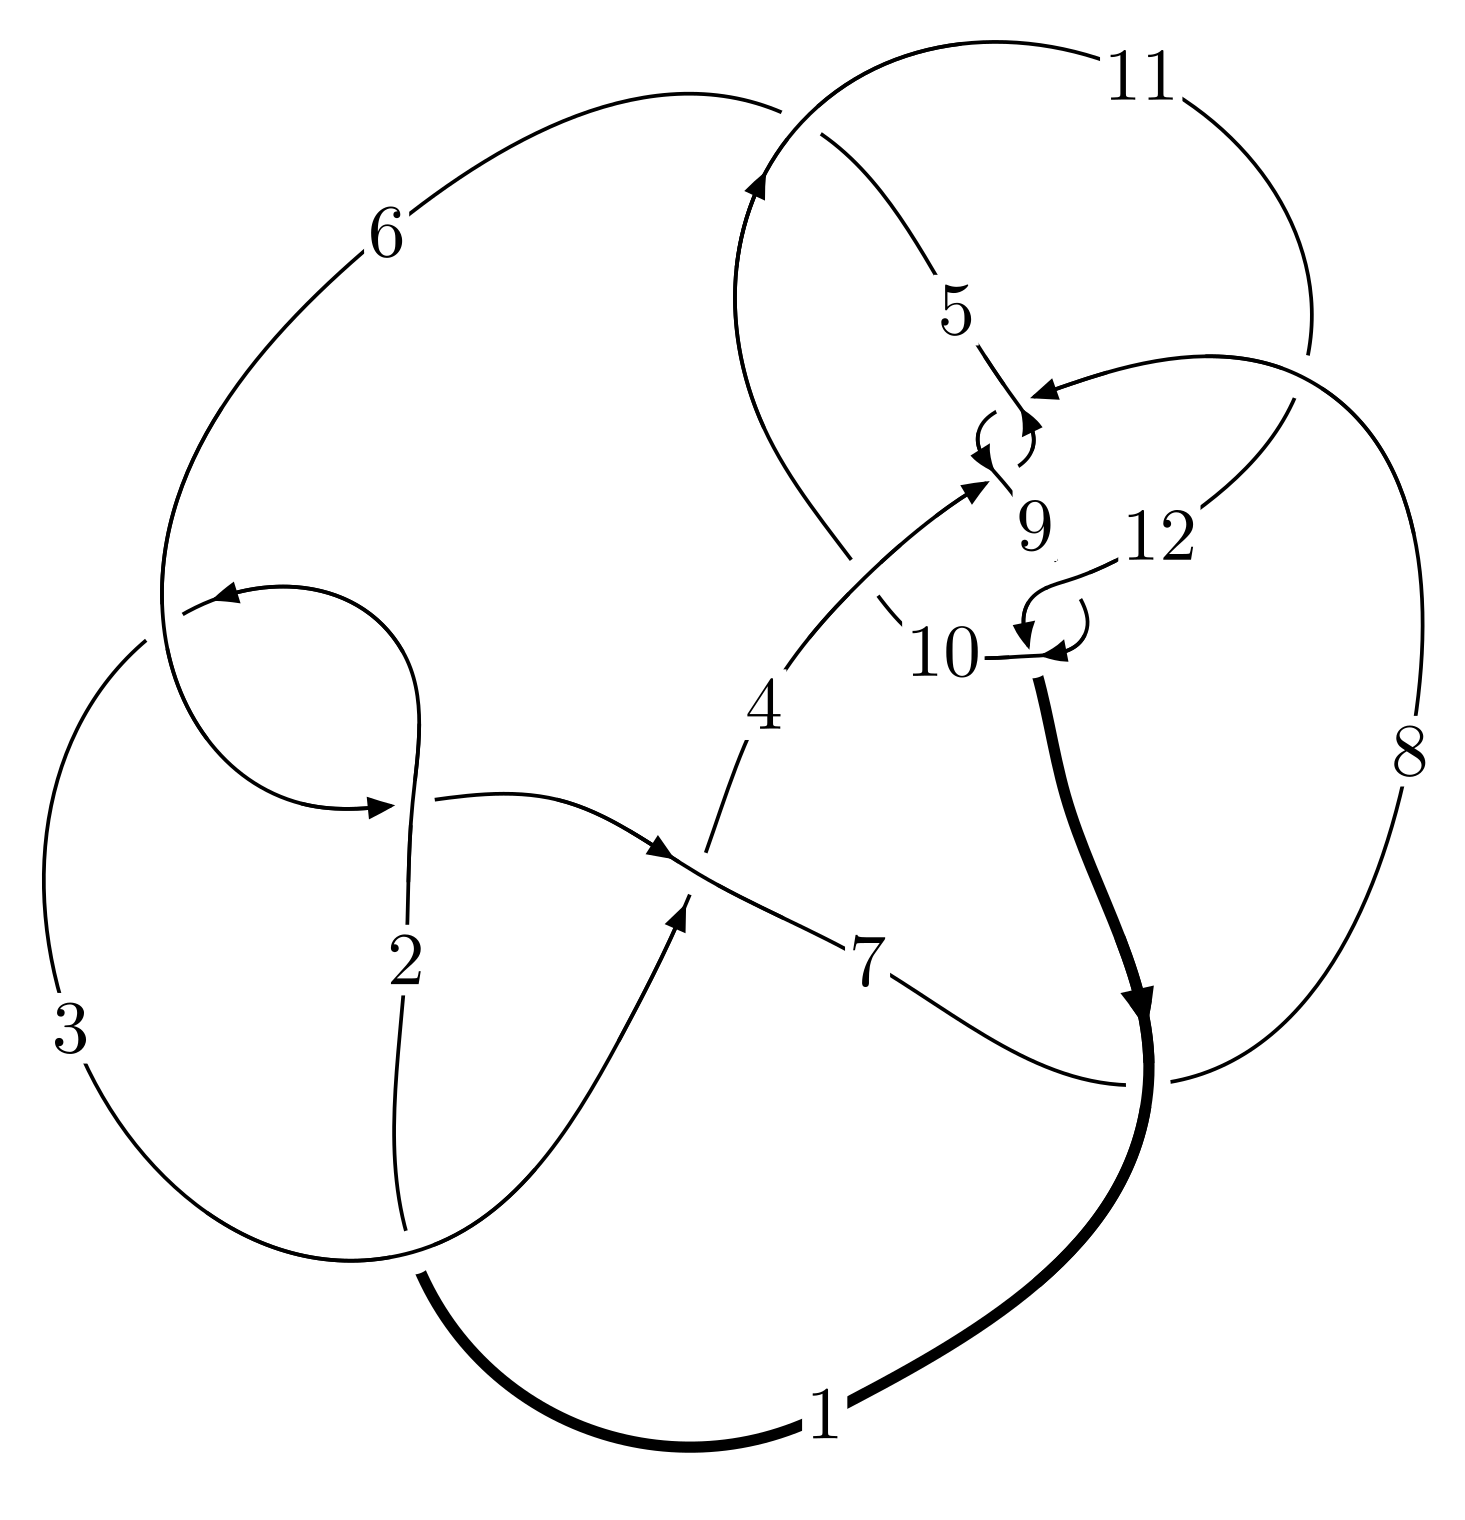
\includegraphics[width=112pt]{../../../GIT/diagram.site/Diagrams/png/1028_12a_0227.png}\\
\ \ \ A knot diagram\footnotemark}&
\allowdisplaybreaks
\textbf{Linearized knot diagam} \\
\cline{2-2}
 &
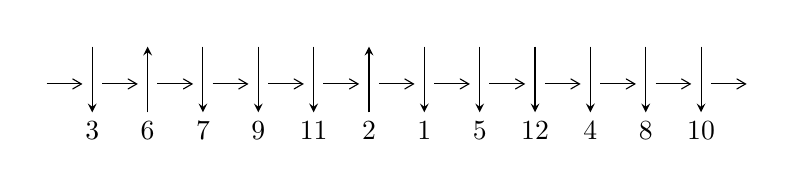
\begin{tikzpicture}[x=20pt, y=17pt]
	% nodes
	\node (C0) at (0, 0) {};
	\node (C1) at (1, 0) {};
	\node (C1U) at (1, +1) {};
	\node (C1D) at (1, -1) {3};

	\node (C2) at (2, 0) {};
	\node (C2U) at (2, +1) {};
	\node (C2D) at (2, -1) {6};

	\node (C3) at (3, 0) {};
	\node (C3U) at (3, +1) {};
	\node (C3D) at (3, -1) {7};

	\node (C4) at (4, 0) {};
	\node (C4U) at (4, +1) {};
	\node (C4D) at (4, -1) {9};

	\node (C5) at (5, 0) {};
	\node (C5U) at (5, +1) {};
	\node (C5D) at (5, -1) {11};

	\node (C6) at (6, 0) {};
	\node (C6U) at (6, +1) {};
	\node (C6D) at (6, -1) {2};

	\node (C7) at (7, 0) {};
	\node (C7U) at (7, +1) {};
	\node (C7D) at (7, -1) {1};

	\node (C8) at (8, 0) {};
	\node (C8U) at (8, +1) {};
	\node (C8D) at (8, -1) {5};

	\node (C9) at (9, 0) {};
	\node (C9U) at (9, +1) {};
	\node (C9D) at (9, -1) {12};

	\node (C10) at (10, 0) {};
	\node (C10U) at (10, +1) {};
	\node (C10D) at (10, -1) {4};

	\node (C11) at (11, 0) {};
	\node (C11U) at (11, +1) {};
	\node (C11D) at (11, -1) {8};

	\node (C12) at (12, 0) {};
	\node (C12U) at (12, +1) {};
	\node (C12D) at (12, -1) {10};
	\node (C13) at (13, 0) {};

	% arrows
	\draw[->,>={angle 60}]
	(C0) edge (C1) (C1) edge (C2) (C2) edge (C3) (C3) edge (C4) (C4) edge (C5) (C5) edge (C6) (C6) edge (C7) (C7) edge (C8) (C8) edge (C9) (C9) edge (C10) (C10) edge (C11) (C11) edge (C12) (C12) edge (C13) ;	\draw[->,>=stealth]
	(C1U) edge (C1D) (C2D) edge (C2U) (C3U) edge (C3D) (C4U) edge (C4D) (C5U) edge (C5D) (C6D) edge (C6U) (C7U) edge (C7D) (C8U) edge (C8D) (C9U) edge (C9D) (C10U) edge (C10D) (C11U) edge (C11D) (C12U) edge (C12D) ;
	\end{tikzpicture} \\
\hhline{~~} \\& 
\textbf{Solving Sequence} \\ \cline{2-2} 
 &
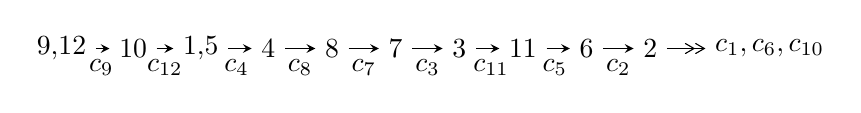
\begin{tikzpicture}[x=23pt, y=7pt]
	% node
	\node (A0) at (-1/8, 0) {9,12};
	\node (A1) at (1, 0) {10};
	\node (A2) at (33/16, 0) {1,5};
	\node (A3) at (25/8, 0) {4};
	\node (A4) at (33/8, 0) {8};
	\node (A5) at (41/8, 0) {7};
	\node (A6) at (49/8, 0) {3};
	\node (A7) at (57/8, 0) {11};
	\node (A8) at (65/8, 0) {6};
	\node (A9) at (73/8, 0) {2};
	\node (C1) at (1/2, -1) {$c_{9}$};
	\node (C2) at (3/2, -1) {$c_{12}$};
	\node (C3) at (21/8, -1) {$c_{4}$};
	\node (C4) at (29/8, -1) {$c_{8}$};
	\node (C5) at (37/8, -1) {$c_{7}$};
	\node (C6) at (45/8, -1) {$c_{3}$};
	\node (C7) at (53/8, -1) {$c_{11}$};
	\node (C8) at (61/8, -1) {$c_{5}$};
	\node (C9) at (69/8, -1) {$c_{2}$};
	\node (A10) at (11, 0) {$c_{1},c_{6},c_{10}$};

	% edge
	\draw[->,>=stealth]	
	(A0) edge (A1) (A1) edge (A2) (A2) edge (A3) (A3) edge (A4) (A4) edge (A5) (A5) edge (A6) (A6) edge (A7) (A7) edge (A8) (A8) edge (A9) ;
	\draw[->>,>={angle 60}]	
	(A9) edge (A10);
\end{tikzpicture} \\ 

\end{tabular} \\

\footnotetext{
The image of knot diagram is generated by the software ``\textbf{Draw programme}" developed by Andrew Bartholomew(\url{http://www.layer8.co.uk/maths/draw/index.htm\#Running-draw}), where we modified some parts for our purpose(\url{https://github.com/CATsTAILs/LinksPainter}).
}\phantom \\ \newline 
\centering \textbf{Ideals for irreducible components\footnotemark of $X_{\text{par}}$} 
 
\begin{align*}
I^u_{1}&=\langle 
4.95039\times10^{487} u^{126}+2.56995\times10^{488} u^{125}+\cdots+6.32406\times10^{487} b-1.63483\times10^{490},\\
\phantom{I^u_{1}}&\phantom{= \langle  }-5.75750\times10^{488} u^{126}-1.83682\times10^{490} u^{125}+\cdots+3.65530\times10^{490} a+4.29408\times10^{492},\\
\phantom{I^u_{1}}&\phantom{= \langle  }u^{127}+6 u^{126}+\cdots-4456 u-289\rangle \\
I^u_{2}&=\langle 
408 a^4+322 a^3+13 a^2+29 b-150 a-27,\;17 a^5+12 a^4-4 a^3-7 a^2+1,\;u-1\rangle \\
\\
\end{align*}
\raggedright * 2 irreducible components of $\dim_{\mathbb{C}}=0$, with total 132 representations.\\
\footnotetext{All coefficients of polynomials are rational numbers. But the coefficients are sometimes approximated in decimal forms when there is not enough margin.}
\newpage
\renewcommand{\arraystretch}{1}
\centering \section*{I. $I^u_{1}= \langle 4.95\times10^{487} u^{126}+2.57\times10^{488} u^{125}+\cdots+6.32\times10^{487} b-1.63\times10^{490},\;-5.76\times10^{488} u^{126}-1.84\times10^{490} u^{125}+\cdots+3.66\times10^{490} a+4.29\times10^{492},\;u^{127}+6 u^{126}+\cdots-4456 u-289 \rangle$}
\flushleft \textbf{(i) Arc colorings}\\
\begin{tabular}{m{7pt} m{180pt} m{7pt} m{180pt} }
\flushright $a_{9}=$&$\begin{pmatrix}1\\0\end{pmatrix}$ \\
\flushright $a_{12}=$&$\begin{pmatrix}0\\u\end{pmatrix}$ \\
\flushright $a_{10}=$&$\begin{pmatrix}1\\u^2\end{pmatrix}$ \\
\flushright $a_{1}=$&$\begin{pmatrix}- u\\- u^3+u\end{pmatrix}$ \\
\flushright $a_{5}=$&$\begin{pmatrix}0.0157511 u^{126}+0.502508 u^{125}+\cdots-1625.76 u-117.475\\-0.782788 u^{126}-4.06377 u^{125}+\cdots+3675.88 u+258.509\end{pmatrix}$ \\
\flushright $a_{4}=$&$\begin{pmatrix}-0.767037 u^{126}-3.56126 u^{125}+\cdots+2050.12 u+141.034\\-0.782788 u^{126}-4.06377 u^{125}+\cdots+3675.88 u+258.509\end{pmatrix}$ \\
\flushright $a_{8}=$&$\begin{pmatrix}0.325046 u^{126}+1.66964 u^{125}+\cdots-1469.09 u-101.084\\1.48773 u^{126}+7.64401 u^{125}+\cdots-6389.62 u-439.447\end{pmatrix}$ \\
\flushright $a_{7}=$&$\begin{pmatrix}1.43965 u^{126}+7.65363 u^{125}+\cdots-7403.82 u-515.811\\0.627650 u^{126}+3.35407 u^{125}+\cdots-3268.21 u-228.073\end{pmatrix}$ \\
\flushright $a_{3}=$&$\begin{pmatrix}0.0752549 u^{126}+0.493597 u^{125}+\cdots-467.578 u-21.8549\\-0.323000 u^{126}-1.55448 u^{125}+\cdots+1076.67 u+75.5079\end{pmatrix}$ \\
\flushright $a_{11}=$&$\begin{pmatrix}0.0868161 u^{126}+0.553087 u^{125}+\cdots-871.738 u-62.8207\\-0.326280 u^{126}-1.32698 u^{125}+\cdots-51.1311 u-12.2547\end{pmatrix}$ \\
\flushright $a_{6}=$&$\begin{pmatrix}0.597942 u^{126}+3.24568 u^{125}+\cdots-3738.93 u-252.966\\-0.343979 u^{126}-1.59473 u^{125}+\cdots+745.172 u+49.8287\end{pmatrix}$ \\
\flushright $a_{2}=$&$\begin{pmatrix}-0.447356 u^{126}-1.94031 u^{125}+\cdots-444.375 u-31.5491\\-0.913367 u^{126}-5.14785 u^{125}+\cdots+6295.33 u+447.308\end{pmatrix}$\\&\end{tabular}
\flushleft \textbf{(ii) Obstruction class $= -1$}\\~\\
\flushleft \textbf{(iii) Cusp Shapes $= -0.841205 u^{126}-6.08545 u^{125}+\cdots+12477.0 u+905.235$}\\~\\
\newpage\renewcommand{\arraystretch}{1}
\flushleft \textbf{(iv) u-Polynomials at the component}\newline \\
\begin{tabular}{m{50pt}|m{274pt}}
Crossings & \hspace{64pt}u-Polynomials at each crossing \\
\hline $$\begin{aligned}c_{1}\end{aligned}$$&$\begin{aligned}
&u^{127}+60 u^{126}+\cdots+2 u-1
\end{aligned}$\\
\hline $$\begin{aligned}c_{2},c_{6}\end{aligned}$$&$\begin{aligned}
&u^{127}-2 u^{126}+\cdots- u^2+1
\end{aligned}$\\
\hline $$\begin{aligned}c_{3}\end{aligned}$$&$\begin{aligned}
&u^{127}+2 u^{126}+\cdots+87846 u+10961
\end{aligned}$\\
\hline $$\begin{aligned}c_{4},c_{8}\end{aligned}$$&$\begin{aligned}
&u^{127}+2 u^{126}+\cdots+4 u+1
\end{aligned}$\\
\hline $$\begin{aligned}c_{5}\end{aligned}$$&$\begin{aligned}
&u^{127}+u^{126}+\cdots+134368 u+9248
\end{aligned}$\\
\hline $$\begin{aligned}c_{7}\end{aligned}$$&$\begin{aligned}
&u^{127}-10 u^{126}+\cdots-28635552 u+3955392
\end{aligned}$\\
\hline $$\begin{aligned}c_{9},c_{12}\end{aligned}$$&$\begin{aligned}
&u^{127}-6 u^{126}+\cdots-4456 u+289
\end{aligned}$\\
\hline $$\begin{aligned}c_{10}\end{aligned}$$&$\begin{aligned}
&17(17 u^{127}+219 u^{126}+\cdots+1318123 u+177763)
\end{aligned}$\\
\hline $$\begin{aligned}c_{11}\end{aligned}$$&$\begin{aligned}
&17(17 u^{127}-213 u^{126}+\cdots-65771 u+7177)
\end{aligned}$\\
\hline
\end{tabular}\\~\\
\newpage\renewcommand{\arraystretch}{1}
\flushleft \textbf{(v) Riley Polynomials at the component}\newline \\
\begin{tabular}{m{50pt}|m{274pt}}
Crossings & \hspace{64pt}Riley Polynomials at each crossing \\
\hline $$\begin{aligned}c_{1}\end{aligned}$$&$\begin{aligned}
&y^{127}+16 y^{126}+\cdots+14 y-1
\end{aligned}$\\
\hline $$\begin{aligned}c_{2},c_{6}\end{aligned}$$&$\begin{aligned}
&y^{127}+60 y^{126}+\cdots+2 y-1
\end{aligned}$\\
\hline $$\begin{aligned}c_{3}\end{aligned}$$&$\begin{aligned}
&y^{127}-28 y^{126}+\cdots+6473657330 y-120143521
\end{aligned}$\\
\hline $$\begin{aligned}c_{4},c_{8}\end{aligned}$$&$\begin{aligned}
&y^{127}+68 y^{126}+\cdots+2 y-1
\end{aligned}$\\
\hline $$\begin{aligned}c_{5}\end{aligned}$$&$\begin{aligned}
&y^{127}+33 y^{126}+\cdots+1848564224 y-85525504
\end{aligned}$\\
\hline $$\begin{aligned}c_{7}\end{aligned}$$&$\begin{aligned}
&y^{127}+36 y^{126}+\cdots-534622349001600 y-15645125873664
\end{aligned}$\\
\hline $$\begin{aligned}c_{9},c_{12}\end{aligned}$$&$\begin{aligned}
&y^{127}-72 y^{126}+\cdots+7252068 y-83521
\end{aligned}$\\
\hline $$\begin{aligned}c_{10}\end{aligned}$$&$\begin{aligned}
&289(289 y^{127}-11547 y^{126}+\cdots-3.38566\times10^{11} y-3.15997\times10^{10})
\end{aligned}$\\
\hline $$\begin{aligned}c_{11}\end{aligned}$$&$\begin{aligned}
&289(289 y^{127}+25283 y^{126}+\cdots-3.86260\times10^{9} y-5.15093\times10^{7})
\end{aligned}$\\
\hline
\end{tabular}\\~\\
\newpage\flushleft \textbf{(vi) Complex Volumes and Cusp Shapes}
$$\begin{array}{c|c|c}  
\text{Solutions to }I^u_{1}& \I (\text{vol} + \sqrt{-1}CS) & \text{Cusp shape}\\
 \hline 
\begin{aligned}
u &= -0.852701 + 0.540301 I \\
a &= -1.34277 - 0.93308 I \\
b &= -0.609646 + 1.164040 I\end{aligned}
 & \phantom{-}5.72289 + 3.58734 I & \phantom{-0.000000 } 0 \\ \hline\begin{aligned}
u &= -0.852701 - 0.540301 I \\
a &= -1.34277 + 0.93308 I \\
b &= -0.609646 - 1.164040 I\end{aligned}
 & \phantom{-}5.72289 - 3.58734 I & \phantom{-0.000000 } 0 \\ \hline\begin{aligned}
u &= -1.014830 + 0.102099 I \\
a &= -0.405389 - 0.081079 I \\
b &= -1.41236 - 0.38918 I\end{aligned}
 & -7.60578 - 4.18983 I & \phantom{-0.000000 } 0 \\ \hline\begin{aligned}
u &= -1.014830 - 0.102099 I \\
a &= -0.405389 + 0.081079 I \\
b &= -1.41236 + 0.38918 I\end{aligned}
 & -7.60578 + 4.18983 I & \phantom{-0.000000 } 0 \\ \hline\begin{aligned}
u &= -0.879964 + 0.429525 I \\
a &= -0.122431 - 0.894058 I \\
b &= \phantom{-}0.32988 + 1.45127 I\end{aligned}
 & \phantom{-}2.31409 + 8.20324 I & \phantom{-0.000000 } 0 \\ \hline\begin{aligned}
u &= -0.879964 - 0.429525 I \\
a &= -0.122431 + 0.894058 I \\
b &= \phantom{-}0.32988 - 1.45127 I\end{aligned}
 & \phantom{-}2.31409 - 8.20324 I & \phantom{-0.000000 } 0 \\ \hline\begin{aligned}
u &= \phantom{-}0.145194 + 0.964926 I \\
a &= \phantom{-}0.20478 + 1.71176 I \\
b &= -0.333801 - 1.133100 I\end{aligned}
 & -0.42685 - 6.05740 I & \phantom{-0.000000 } 0 \\ \hline\begin{aligned}
u &= \phantom{-}0.145194 - 0.964926 I \\
a &= \phantom{-}0.20478 - 1.71176 I \\
b &= -0.333801 + 1.133100 I\end{aligned}
 & -0.42685 + 6.05740 I & \phantom{-0.000000 } 0 \\ \hline\begin{aligned}
u &= \phantom{-}0.966417 + 0.023996 I \\
a &= -6.60150 + 0.91190 I \\
b &= -0.071131 - 0.985873 I\end{aligned}
 & -1.82223 - 0.98089 I & \phantom{-0.000000 } 0 \\ \hline\begin{aligned}
u &= \phantom{-}0.966417 - 0.023996 I \\
a &= -6.60150 - 0.91190 I \\
b &= -0.071131 + 0.985873 I\end{aligned}
 & -1.82223 + 0.98089 I & \phantom{-0.000000 } 0\\
 \hline 
 \end{array}$$\newpage$$\begin{array}{c|c|c}  
\text{Solutions to }I^u_{1}& \I (\text{vol} + \sqrt{-1}CS) & \text{Cusp shape}\\
 \hline 
\begin{aligned}
u &= -1.026420 + 0.175064 I \\
a &= \phantom{-}0.374744 + 0.152595 I \\
b &= \phantom{-}1.268490 + 0.333071 I\end{aligned}
 & -4.30492 + 0.43151 I & \phantom{-0.000000 } 0 \\ \hline\begin{aligned}
u &= -1.026420 - 0.175064 I \\
a &= \phantom{-}0.374744 - 0.152595 I \\
b &= \phantom{-}1.268490 - 0.333071 I\end{aligned}
 & -4.30492 - 0.43151 I & \phantom{-0.000000 } 0 \\ \hline\begin{aligned}
u &= \phantom{-}0.896921 + 0.533977 I \\
a &= \phantom{-}0.294430 - 0.441663 I \\
b &= -0.424264 + 0.189155 I\end{aligned}
 & -2.29093 + 3.74594 I & \phantom{-0.000000 } 0 \\ \hline\begin{aligned}
u &= \phantom{-}0.896921 - 0.533977 I \\
a &= \phantom{-}0.294430 + 0.441663 I \\
b &= -0.424264 - 0.189155 I\end{aligned}
 & -2.29093 - 3.74594 I & \phantom{-0.000000 } 0 \\ \hline\begin{aligned}
u &= -0.609834 + 0.717118 I \\
a &= -0.339685 - 1.133880 I \\
b &= \phantom{-}0.323059 + 1.314320 I\end{aligned}
 & \phantom{-}5.29418 - 3.85660 I & \phantom{-0.000000 } 0 \\ \hline\begin{aligned}
u &= -0.609834 - 0.717118 I \\
a &= -0.339685 + 1.133880 I \\
b &= \phantom{-}0.323059 - 1.314320 I\end{aligned}
 & \phantom{-}5.29418 + 3.85660 I & \phantom{-0.000000 } 0 \\ \hline\begin{aligned}
u &= -0.817941 + 0.452259 I \\
a &= \phantom{-}0.179258 + 0.897431 I \\
b &= -0.31067 - 1.42866 I\end{aligned}
 & \phantom{-}4.69061 + 3.13207 I & \phantom{-0.000000 } 0 \\ \hline\begin{aligned}
u &= -0.817941 - 0.452259 I \\
a &= \phantom{-}0.179258 - 0.897431 I \\
b &= -0.31067 + 1.42866 I\end{aligned}
 & \phantom{-}4.69061 - 3.13207 I & \phantom{-0.000000 } 0 \\ \hline\begin{aligned}
u &= -0.911216 + 0.575095 I \\
a &= \phantom{-}1.27057 + 1.00453 I \\
b &= \phantom{-}0.604539 - 1.190270 I\end{aligned}
 & \phantom{-}4.39753 + 8.75064 I & \phantom{-0.000000 } 0 \\ \hline\begin{aligned}
u &= -0.911216 - 0.575095 I \\
a &= \phantom{-}1.27057 - 1.00453 I \\
b &= \phantom{-}0.604539 + 1.190270 I\end{aligned}
 & \phantom{-}4.39753 - 8.75064 I & \phantom{-0.000000 } 0\\
 \hline 
 \end{array}$$\newpage$$\begin{array}{c|c|c}  
\text{Solutions to }I^u_{1}& \I (\text{vol} + \sqrt{-1}CS) & \text{Cusp shape}\\
 \hline 
\begin{aligned}
u &= \phantom{-}0.668794 + 0.850025 I \\
a &= -0.29873 + 1.74665 I \\
b &= -0.326607 - 1.027610 I\end{aligned}
 & -0.091432 + 0.584746 I & \phantom{-0.000000 } 0 \\ \hline\begin{aligned}
u &= \phantom{-}0.668794 - 0.850025 I \\
a &= -0.29873 - 1.74665 I \\
b &= -0.326607 + 1.027610 I\end{aligned}
 & -0.091432 - 0.584746 I & \phantom{-0.000000 } 0 \\ \hline\begin{aligned}
u &= -0.679771 + 0.609705 I \\
a &= \phantom{-}0.309119 + 1.029780 I \\
b &= -0.310849 - 1.350500 I\end{aligned}
 & \phantom{-}6.23156 + 0.94338 I & \phantom{-0.000000 } 0 \\ \hline\begin{aligned}
u &= -0.679771 - 0.609705 I \\
a &= \phantom{-}0.309119 - 1.029780 I \\
b &= -0.310849 + 1.350500 I\end{aligned}
 & \phantom{-}6.23156 - 0.94338 I & \phantom{-0.000000 } 0 \\ \hline\begin{aligned}
u &= -0.838598 + 0.355662 I \\
a &= \phantom{-}1.253440 + 0.620849 I \\
b &= \phantom{-}0.697957 - 1.121430 I\end{aligned}
 & -0.19206 + 2.87859 I & \phantom{-0.000000 } 0 \\ \hline\begin{aligned}
u &= -0.838598 - 0.355662 I \\
a &= \phantom{-}1.253440 - 0.620849 I \\
b &= \phantom{-}0.697957 + 1.121430 I\end{aligned}
 & -0.19206 - 2.87859 I & \phantom{-0.000000 } 0 \\ \hline\begin{aligned}
u &= \phantom{-}0.905744 + 0.042812 I \\
a &= -4.35368 - 4.03692 I \\
b &= -0.098574 + 1.035330 I\end{aligned}
 & \phantom{-}0.22852 - 5.78675 I & \phantom{-0.000000 } 0 \\ \hline\begin{aligned}
u &= \phantom{-}0.905744 - 0.042812 I \\
a &= -4.35368 + 4.03692 I \\
b &= -0.098574 - 1.035330 I\end{aligned}
 & \phantom{-}0.22852 + 5.78675 I & \phantom{-0.000000 } 0 \\ \hline\begin{aligned}
u &= \phantom{-}1.020750 + 0.410520 I \\
a &= -0.229262 + 0.389474 I \\
b &= \phantom{-}0.362254 - 0.230244 I\end{aligned}
 & -0.531400 - 0.664928 I & \phantom{-0.000000 } 0 \\ \hline\begin{aligned}
u &= \phantom{-}1.020750 - 0.410520 I \\
a &= -0.229262 - 0.389474 I \\
b &= \phantom{-}0.362254 + 0.230244 I\end{aligned}
 & -0.531400 + 0.664928 I & \phantom{-0.000000 } 0\\
 \hline 
 \end{array}$$\newpage$$\begin{array}{c|c|c}  
\text{Solutions to }I^u_{1}& \I (\text{vol} + \sqrt{-1}CS) & \text{Cusp shape}\\
 \hline 
\begin{aligned}
u &= \phantom{-}0.874294 + 0.018592 I \\
a &= \phantom{-}3.98628 + 3.44373 I \\
b &= \phantom{-}0.112976 - 1.026810 I\end{aligned}
 & \phantom{-}2.20337 - 0.95953 I & \phantom{-0.000000 } 0 \\ \hline\begin{aligned}
u &= \phantom{-}0.874294 - 0.018592 I \\
a &= \phantom{-}3.98628 - 3.44373 I \\
b &= \phantom{-}0.112976 + 1.026810 I\end{aligned}
 & \phantom{-}2.20337 + 0.95953 I & \phantom{-0.000000 } 0 \\ \hline\begin{aligned}
u &= -1.029780 + 0.468480 I \\
a &= \phantom{-}0.225034 + 0.332957 I \\
b &= \phantom{-}1.045950 + 0.219050 I\end{aligned}
 & \phantom{-}0.012322 + 0.568494 I & \phantom{-0.000000 } 0 \\ \hline\begin{aligned}
u &= -1.029780 - 0.468480 I \\
a &= \phantom{-}0.225034 - 0.332957 I \\
b &= \phantom{-}1.045950 - 0.219050 I\end{aligned}
 & \phantom{-}0.012322 - 0.568494 I & \phantom{-0.000000 } 0 \\ \hline\begin{aligned}
u &= -1.124280 + 0.180795 I \\
a &= -0.294506 - 0.129350 I \\
b &= -1.261790 - 0.205517 I\end{aligned}
 & -8.09446 + 4.49424 I & \phantom{-0.000000 } 0 \\ \hline\begin{aligned}
u &= -1.124280 - 0.180795 I \\
a &= -0.294506 + 0.129350 I \\
b &= -1.261790 + 0.205517 I\end{aligned}
 & -8.09446 - 4.49424 I & \phantom{-0.000000 } 0 \\ \hline\begin{aligned}
u &= -0.717437 + 0.463098 I \\
a &= -1.55187 - 0.74544 I \\
b &= -0.607863 + 1.091750 I\end{aligned}
 & \phantom{-}4.97586 + 0.74438 I & \phantom{-0.000000 } 0 \\ \hline\begin{aligned}
u &= -0.717437 - 0.463098 I \\
a &= -1.55187 + 0.74544 I \\
b &= -0.607863 - 1.091750 I\end{aligned}
 & \phantom{-}4.97586 - 0.74438 I & \phantom{-0.000000 } 0 \\ \hline\begin{aligned}
u &= -0.029470 + 0.837233 I \\
a &= -0.217734 + 0.748893 I \\
b &= \phantom{-}0.652250 + 0.043201 I\end{aligned}
 & \phantom{-}0.53107 - 8.60738 I & \phantom{-0.000000 } 0 \\ \hline\begin{aligned}
u &= -0.029470 - 0.837233 I \\
a &= -0.217734 - 0.748893 I \\
b &= \phantom{-}0.652250 - 0.043201 I\end{aligned}
 & \phantom{-}0.53107 + 8.60738 I & \phantom{-0.000000 } 0\\
 \hline 
 \end{array}$$\newpage$$\begin{array}{c|c|c}  
\text{Solutions to }I^u_{1}& \I (\text{vol} + \sqrt{-1}CS) & \text{Cusp shape}\\
 \hline 
\begin{aligned}
u &= -0.408417 + 1.106130 I \\
a &= -0.253561 - 1.380940 I \\
b &= \phantom{-}0.377568 + 1.233580 I\end{aligned}
 & \phantom{-}5.96486 - 0.16558 I & \phantom{-0.000000 } 0 \\ \hline\begin{aligned}
u &= -0.408417 - 1.106130 I \\
a &= -0.253561 + 1.380940 I \\
b &= \phantom{-}0.377568 - 1.233580 I\end{aligned}
 & \phantom{-}5.96486 + 0.16558 I & \phantom{-0.000000 } 0 \\ \hline\begin{aligned}
u &= -0.755531 + 0.316294 I \\
a &= -0.194572 - 0.752235 I \\
b &= \phantom{-}0.24174 + 1.46206 I\end{aligned}
 & \phantom{-}0.096131 + 0.260592 I & \phantom{-0.000000 } 0 \\ \hline\begin{aligned}
u &= -0.755531 - 0.316294 I \\
a &= -0.194572 + 0.752235 I \\
b &= \phantom{-}0.24174 - 1.46206 I\end{aligned}
 & \phantom{-}0.096131 - 0.260592 I & \phantom{-0.000000 } 0 \\ \hline\begin{aligned}
u &= -1.101670 + 0.487832 I \\
a &= -0.188407 - 0.304665 I \\
b &= -1.059130 - 0.185882 I\end{aligned}
 & \phantom{-}0.86608 + 5.64943 I & \phantom{-0.000000 } 0 \\ \hline\begin{aligned}
u &= -1.101670 - 0.487832 I \\
a &= -0.188407 + 0.304665 I \\
b &= -1.059130 + 0.185882 I\end{aligned}
 & \phantom{-}0.86608 - 5.64943 I & \phantom{-0.000000 } 0 \\ \hline\begin{aligned}
u &= -0.648207 + 0.444177 I \\
a &= \phantom{-}1.69452 + 0.67956 I \\
b &= \phantom{-}0.589917 - 1.058670 I\end{aligned}
 & \phantom{-}2.97420 - 4.45774 I & \phantom{-0.000000 } 0 \\ \hline\begin{aligned}
u &= -0.648207 - 0.444177 I \\
a &= \phantom{-}1.69452 - 0.67956 I \\
b &= \phantom{-}0.589917 + 1.058670 I\end{aligned}
 & \phantom{-}2.97420 + 4.45774 I & \phantom{-0.000000 } 0 \\ \hline\begin{aligned}
u &= -0.353742 + 1.162250 I \\
a &= \phantom{-}0.23638 + 1.40821 I \\
b &= -0.383655 - 1.220840 I\end{aligned}
 & \phantom{-}7.21684 - 5.07057 I & \phantom{-0.000000 } 0 \\ \hline\begin{aligned}
u &= -0.353742 - 1.162250 I \\
a &= \phantom{-}0.23638 - 1.40821 I \\
b &= -0.383655 + 1.220840 I\end{aligned}
 & \phantom{-}7.21684 + 5.07057 I & \phantom{-0.000000 } 0\\
 \hline 
 \end{array}$$\newpage$$\begin{array}{c|c|c}  
\text{Solutions to }I^u_{1}& \I (\text{vol} + \sqrt{-1}CS) & \text{Cusp shape}\\
 \hline 
\begin{aligned}
u &= -0.070426 + 0.781275 I \\
a &= \phantom{-}0.200965 - 0.782956 I \\
b &= -0.648612 - 0.067576 I\end{aligned}
 & \phantom{-}2.60757 - 3.58583 I & \phantom{-0.000000 } 0 \\ \hline\begin{aligned}
u &= -0.070426 - 0.781275 I \\
a &= \phantom{-}0.200965 + 0.782956 I \\
b &= -0.648612 + 0.067576 I\end{aligned}
 & \phantom{-}2.60757 + 3.58583 I & \phantom{-0.000000 } 0 \\ \hline\begin{aligned}
u &= -0.183040 + 1.202740 I \\
a &= -0.21628 - 1.47407 I \\
b &= \phantom{-}0.382764 + 1.190200 I\end{aligned}
 & \phantom{-}1.56779 - 5.07438 I & \phantom{-0.000000 } 0 \\ \hline\begin{aligned}
u &= -0.183040 - 1.202740 I \\
a &= -0.21628 + 1.47407 I \\
b &= \phantom{-}0.382764 - 1.190200 I\end{aligned}
 & \phantom{-}1.56779 + 5.07438 I & \phantom{-0.000000 } 0 \\ \hline\begin{aligned}
u &= \phantom{-}1.209210 + 0.230205 I \\
a &= -0.872059 + 0.432961 I \\
b &= -0.197040 - 0.810735 I\end{aligned}
 & -1.06593 - 1.10261 I & \phantom{-0.000000 } 0 \\ \hline\begin{aligned}
u &= \phantom{-}1.209210 - 0.230205 I \\
a &= -0.872059 - 0.432961 I \\
b &= -0.197040 + 0.810735 I\end{aligned}
 & -1.06593 + 1.10261 I & \phantom{-0.000000 } 0 \\ \hline\begin{aligned}
u &= \phantom{-}0.896049 + 0.853495 I \\
a &= \phantom{-}0.41426 - 1.53788 I \\
b &= \phantom{-}0.341377 + 0.982621 I\end{aligned}
 & \phantom{-}1.31495 - 3.76899 I & \phantom{-0.000000 } 0 \\ \hline\begin{aligned}
u &= \phantom{-}0.896049 - 0.853495 I \\
a &= \phantom{-}0.41426 + 1.53788 I \\
b &= \phantom{-}0.341377 - 0.982621 I\end{aligned}
 & \phantom{-}1.31495 + 3.76899 I & \phantom{-0.000000 } 0 \\ \hline\begin{aligned}
u &= \phantom{-}0.560206 + 0.515752 I \\
a &= \phantom{-}0.451441 - 0.515159 I \\
b &= -0.458401 + 0.075256 I\end{aligned}
 & -3.32415 - 2.87892 I & \phantom{-0.000000 } 0 \\ \hline\begin{aligned}
u &= \phantom{-}0.560206 - 0.515752 I \\
a &= \phantom{-}0.451441 + 0.515159 I \\
b &= -0.458401 - 0.075256 I\end{aligned}
 & -3.32415 + 2.87892 I & \phantom{-0.000000 } 0\\
 \hline 
 \end{array}$$\newpage$$\begin{array}{c|c|c}  
\text{Solutions to }I^u_{1}& \I (\text{vol} + \sqrt{-1}CS) & \text{Cusp shape}\\
 \hline 
\begin{aligned}
u &= \phantom{-}0.751197 + 0.024211 I \\
a &= \phantom{-}2.79279 - 3.22065 I \\
b &= \phantom{-}0.152354 + 1.028160 I\end{aligned}
 & \phantom{-}2.52127 - 0.93793 I & \phantom{-0.000000 } 0 \\ \hline\begin{aligned}
u &= \phantom{-}0.751197 - 0.024211 I \\
a &= \phantom{-}2.79279 + 3.22065 I \\
b &= \phantom{-}0.152354 - 1.028160 I\end{aligned}
 & \phantom{-}2.52127 + 0.93793 I & \phantom{-0.000000 } 0 \\ \hline\begin{aligned}
u &= -1.201760 + 0.399307 I \\
a &= -0.847325 - 0.984650 I \\
b &= -0.65214 + 1.30518 I\end{aligned}
 & -4.26341 + 2.69423 I & \phantom{-0.000000 } 0 \\ \hline\begin{aligned}
u &= -1.201760 - 0.399307 I \\
a &= -0.847325 + 0.984650 I \\
b &= -0.65214 - 1.30518 I\end{aligned}
 & -4.26341 - 2.69423 I & \phantom{-0.000000 } 0 \\ \hline\begin{aligned}
u &= -0.028343 + 0.729196 I \\
a &= -0.54338 - 1.72726 I \\
b &= \phantom{-}0.283010 + 1.170220 I\end{aligned}
 & \phantom{-}2.32539 - 2.52729 I & \phantom{-0.000000 } 0 \\ \hline\begin{aligned}
u &= -0.028343 - 0.729196 I \\
a &= -0.54338 + 1.72726 I \\
b &= \phantom{-}0.283010 - 1.170220 I\end{aligned}
 & \phantom{-}2.32539 + 2.52729 I & \phantom{-0.000000 } 0 \\ \hline\begin{aligned}
u &= -1.211370 + 0.427564 I \\
a &= \phantom{-}0.169366 + 0.237297 I \\
b &= \phantom{-}1.101290 + 0.152960 I\end{aligned}
 & -5.61618 + 5.48676 I & \phantom{-0.000000 } 0 \\ \hline\begin{aligned}
u &= -1.211370 - 0.427564 I \\
a &= \phantom{-}0.169366 - 0.237297 I \\
b &= \phantom{-}1.101290 - 0.152960 I\end{aligned}
 & -5.61618 - 5.48676 I & \phantom{-0.000000 } 0 \\ \hline\begin{aligned}
u &= -0.353933 + 0.620488 I \\
a &= \phantom{-}0.041314 + 0.841105 I \\
b &= \phantom{-}0.706967 + 0.191328 I\end{aligned}
 & \phantom{-}1.87141 + 3.67539 I & \phantom{-0.000000 } 0 \\ \hline\begin{aligned}
u &= -0.353933 - 0.620488 I \\
a &= \phantom{-}0.041314 - 0.841105 I \\
b &= \phantom{-}0.706967 - 0.191328 I\end{aligned}
 & \phantom{-}1.87141 - 3.67539 I & \phantom{-0.000000 } 0\\
 \hline 
 \end{array}$$\newpage$$\begin{array}{c|c|c}  
\text{Solutions to }I^u_{1}& \I (\text{vol} + \sqrt{-1}CS) & \text{Cusp shape}\\
 \hline 
\begin{aligned}
u &= -0.271409 + 1.257460 I \\
a &= \phantom{-}0.20297 + 1.43887 I \\
b &= -0.395164 - 1.202670 I\end{aligned}
 & \phantom{-}6.24468 - 7.44634 I & \phantom{-0.000000 } 0 \\ \hline\begin{aligned}
u &= -0.271409 - 1.257460 I \\
a &= \phantom{-}0.20297 - 1.43887 I \\
b &= -0.395164 + 1.202670 I\end{aligned}
 & \phantom{-}6.24468 + 7.44634 I & \phantom{-0.000000 } 0 \\ \hline\begin{aligned}
u &= -1.198690 + 0.467402 I \\
a &= \phantom{-}0.897126 + 1.037910 I \\
b &= \phantom{-}0.63347 - 1.29188 I\end{aligned}
 & -1.03817 + 6.95015 I & \phantom{-0.000000 } 0 \\ \hline\begin{aligned}
u &= -1.198690 - 0.467402 I \\
a &= \phantom{-}0.897126 - 1.037910 I \\
b &= \phantom{-}0.63347 + 1.29188 I\end{aligned}
 & -1.03817 - 6.95015 I & \phantom{-0.000000 } 0 \\ \hline\begin{aligned}
u &= -0.237781 + 0.665114 I \\
a &= \phantom{-}0.071797 - 0.855025 I \\
b &= -0.670987 - 0.146539 I\end{aligned}
 & \phantom{-}3.30781 - 1.25100 I & \phantom{-0.000000 } 0 \\ \hline\begin{aligned}
u &= -0.237781 - 0.665114 I \\
a &= \phantom{-}0.071797 + 0.855025 I \\
b &= -0.670987 + 0.146539 I\end{aligned}
 & \phantom{-}3.30781 + 1.25100 I & \phantom{-0.000000 } 0 \\ \hline\begin{aligned}
u &= -1.208050 + 0.491552 I \\
a &= -0.148140 - 0.263017 I \\
b &= -1.077310 - 0.146919 I\end{aligned}
 & -0.71550 + 8.27093 I & \phantom{-0.000000 } 0 \\ \hline\begin{aligned}
u &= -1.208050 - 0.491552 I \\
a &= -0.148140 + 0.263017 I \\
b &= -1.077310 + 0.146919 I\end{aligned}
 & -0.71550 - 8.27093 I & \phantom{-0.000000 } 0 \\ \hline\begin{aligned}
u &= -0.252316 + 1.296670 I \\
a &= -0.18984 - 1.44321 I \\
b &= \phantom{-}0.400598 + 1.198070 I\end{aligned}
 & \phantom{-}4.09272 - 12.51100 I & \phantom{-0.000000 } 0 \\ \hline\begin{aligned}
u &= -0.252316 - 1.296670 I \\
a &= -0.18984 + 1.44321 I \\
b &= \phantom{-}0.400598 - 1.198070 I\end{aligned}
 & \phantom{-}4.09272 + 12.51100 I & \phantom{-0.000000 } 0\\
 \hline 
 \end{array}$$\newpage$$\begin{array}{c|c|c}  
\text{Solutions to }I^u_{1}& \I (\text{vol} + \sqrt{-1}CS) & \text{Cusp shape}\\
 \hline 
\begin{aligned}
u &= \phantom{-}0.083628 + 0.673445 I \\
a &= -0.322639 + 0.808199 I \\
b &= \phantom{-}0.580249 + 0.049725 I\end{aligned}
 & -1.95208 - 1.41580 I & \phantom{-0.000000 } 0 \\ \hline\begin{aligned}
u &= \phantom{-}0.083628 - 0.673445 I \\
a &= -0.322639 - 0.808199 I \\
b &= \phantom{-}0.580249 - 0.049725 I\end{aligned}
 & -1.95208 + 1.41580 I & \phantom{-0.000000 } 0 \\ \hline\begin{aligned}
u &= \phantom{-}1.260780 + 0.407052 I \\
a &= -0.128975 + 0.444802 I \\
b &= \phantom{-}0.366914 - 0.346876 I\end{aligned}
 & -1.11053 - 2.13759 I & \phantom{-0.000000 } 0 \\ \hline\begin{aligned}
u &= \phantom{-}1.260780 - 0.407052 I \\
a &= -0.128975 - 0.444802 I \\
b &= \phantom{-}0.366914 + 0.346876 I\end{aligned}
 & -1.11053 + 2.13759 I & \phantom{-0.000000 } 0 \\ \hline\begin{aligned}
u &= -1.238570 + 0.498015 I \\
a &= \phantom{-}0.135097 + 0.254706 I \\
b &= \phantom{-}1.078830 + 0.136046 I\end{aligned}
 & -3.03620 + 13.45980 I & \phantom{-0.000000 } 0 \\ \hline\begin{aligned}
u &= -1.238570 - 0.498015 I \\
a &= \phantom{-}0.135097 - 0.254706 I \\
b &= \phantom{-}1.078830 - 0.136046 I\end{aligned}
 & -3.03620 - 13.45980 I & \phantom{-0.000000 } 0 \\ \hline\begin{aligned}
u &= \phantom{-}0.651572 + 0.009687 I \\
a &= -2.39930 + 3.54321 I \\
b &= -0.167469 - 1.039610 I\end{aligned}
 & \phantom{-}0.80850 - 5.62228 I & -8.00000 + 6.14117 I \\ \hline\begin{aligned}
u &= \phantom{-}0.651572 - 0.009687 I \\
a &= -2.39930 - 3.54321 I \\
b &= -0.167469 + 1.039610 I\end{aligned}
 & \phantom{-}0.80850 + 5.62228 I & -8.00000 - 6.14117 I \\ \hline\begin{aligned}
u &= -1.265070 + 0.472844 I \\
a &= -0.848771 - 1.083270 I \\
b &= -0.62201 + 1.30751 I\end{aligned}
 & -4.55047 + 10.90910 I & \phantom{-0.000000 } 0 \\ \hline\begin{aligned}
u &= -1.265070 - 0.472844 I \\
a &= -0.848771 + 1.083270 I \\
b &= -0.62201 - 1.30751 I\end{aligned}
 & -4.55047 - 10.90910 I & \phantom{-0.000000 } 0\\
 \hline 
 \end{array}$$\newpage$$\begin{array}{c|c|c}  
\text{Solutions to }I^u_{1}& \I (\text{vol} + \sqrt{-1}CS) & \text{Cusp shape}\\
 \hline 
\begin{aligned}
u &= -1.210730 + 0.659204 I \\
a &= \phantom{-}0.98061 + 1.20435 I \\
b &= \phantom{-}0.585204 - 1.278490 I\end{aligned}
 & \phantom{-}3.36662 + 6.40956 I & \phantom{-0.000000 } 0 \\ \hline\begin{aligned}
u &= -1.210730 - 0.659204 I \\
a &= \phantom{-}0.98061 - 1.20435 I \\
b &= \phantom{-}0.585204 + 1.278490 I\end{aligned}
 & \phantom{-}3.36662 - 6.40956 I & \phantom{-0.000000 } 0 \\ \hline\begin{aligned}
u &= \phantom{-}1.342020 + 0.379840 I \\
a &= -0.583833 + 0.781666 I \\
b &= -0.290946 - 0.805939 I\end{aligned}
 & -1.11970 - 1.03596 I & \phantom{-0.000000 } 0 \\ \hline\begin{aligned}
u &= \phantom{-}1.342020 - 0.379840 I \\
a &= -0.583833 - 0.781666 I \\
b &= -0.290946 + 0.805939 I\end{aligned}
 & -1.11970 + 1.03596 I & \phantom{-0.000000 } 0 \\ \hline\begin{aligned}
u &= \phantom{-}1.326160 + 0.441251 I \\
a &= \phantom{-}0.120414 - 0.474901 I \\
b &= -0.391107 + 0.370722 I\end{aligned}
 & -3.25281 - 6.89189 I & \phantom{-0.000000 } 0 \\ \hline\begin{aligned}
u &= \phantom{-}1.326160 - 0.441251 I \\
a &= \phantom{-}0.120414 + 0.474901 I \\
b &= -0.391107 - 0.370722 I\end{aligned}
 & -3.25281 + 6.89189 I & \phantom{-0.000000 } 0 \\ \hline\begin{aligned}
u &= \phantom{-}1.368300 + 0.296535 I \\
a &= \phantom{-}0.055203 - 0.452326 I \\
b &= -0.336674 + 0.419621 I\end{aligned}
 & -5.07869 + 0.30171 I & \phantom{-0.000000 } 0 \\ \hline\begin{aligned}
u &= \phantom{-}1.368300 - 0.296535 I \\
a &= \phantom{-}0.055203 + 0.452326 I \\
b &= -0.336674 - 0.419621 I\end{aligned}
 & -5.07869 - 0.30171 I & \phantom{-0.000000 } 0 \\ \hline\begin{aligned}
u &= -1.25122 + 0.66759 I \\
a &= -0.95105 - 1.22530 I \\
b &= -0.581822 + 1.286560 I\end{aligned}
 & \phantom{-}4.32872 + 11.49530 I & \phantom{-0.000000 } 0 \\ \hline\begin{aligned}
u &= -1.25122 - 0.66759 I \\
a &= -0.95105 + 1.22530 I \\
b &= -0.581822 - 1.286560 I\end{aligned}
 & \phantom{-}4.32872 - 11.49530 I & \phantom{-0.000000 } 0\\
 \hline 
 \end{array}$$\newpage$$\begin{array}{c|c|c}  
\text{Solutions to }I^u_{1}& \I (\text{vol} + \sqrt{-1}CS) & \text{Cusp shape}\\
 \hline 
\begin{aligned}
u &= \phantom{-}1.08470 + 0.93222 I \\
a &= \phantom{-}0.36108 - 1.37118 I \\
b &= \phantom{-}0.373143 + 0.953420 I\end{aligned}
 & \phantom{-}0.41231 - 5.47477 I & \phantom{-0.000000 } 0 \\ \hline\begin{aligned}
u &= \phantom{-}1.08470 - 0.93222 I \\
a &= \phantom{-}0.36108 + 1.37118 I \\
b &= \phantom{-}0.373143 - 0.953420 I\end{aligned}
 & \phantom{-}0.41231 + 5.47477 I & \phantom{-0.000000 } 0 \\ \hline\begin{aligned}
u &= \phantom{-}1.18333 + 0.84536 I \\
a &= -0.409604 + 1.282880 I \\
b &= -0.367940 - 0.925587 I\end{aligned}
 & -3.80312 - 2.99685 I & \phantom{-0.000000 } 0 \\ \hline\begin{aligned}
u &= \phantom{-}1.18333 - 0.84536 I \\
a &= -0.409604 - 1.282880 I \\
b &= -0.367940 + 0.925587 I\end{aligned}
 & -3.80312 + 2.99685 I & \phantom{-0.000000 } 0 \\ \hline\begin{aligned}
u &= -1.31677 + 0.62741 I \\
a &= \phantom{-}0.88756 + 1.21991 I \\
b &= \phantom{-}0.58569 - 1.30127 I\end{aligned}
 & -2.01313 + 11.43770 I & \phantom{-0.000000 } 0 \\ \hline\begin{aligned}
u &= -1.31677 - 0.62741 I \\
a &= \phantom{-}0.88756 - 1.21991 I \\
b &= \phantom{-}0.58569 + 1.30127 I\end{aligned}
 & -2.01313 - 11.43770 I & \phantom{-0.000000 } 0 \\ \hline\begin{aligned}
u &= -1.31563 + 0.66936 I \\
a &= -0.90391 - 1.24906 I \\
b &= -0.57835 + 1.29849 I\end{aligned}
 & \phantom{-}2.8882 + 14.1361 I & \phantom{-0.000000 } 0 \\ \hline\begin{aligned}
u &= -1.31563 - 0.66936 I \\
a &= -0.90391 + 1.24906 I \\
b &= -0.57835 - 1.29849 I\end{aligned}
 & \phantom{-}2.8882 - 14.1361 I & \phantom{-0.000000 } 0 \\ \hline\begin{aligned}
u &= \phantom{-}1.34735 + 0.60684 I \\
a &= \phantom{-}0.486164 - 1.038140 I \\
b &= \phantom{-}0.345625 + 0.856806 I\end{aligned}
 & -4.52009 - 3.74465 I & \phantom{-0.000000 } 0 \\ \hline\begin{aligned}
u &= \phantom{-}1.34735 - 0.60684 I \\
a &= \phantom{-}0.486164 + 1.038140 I \\
b &= \phantom{-}0.345625 - 0.856806 I\end{aligned}
 & -4.52009 + 3.74465 I & \phantom{-0.000000 } 0\\
 \hline 
 \end{array}$$\newpage$$\begin{array}{c|c|c}  
\text{Solutions to }I^u_{1}& \I (\text{vol} + \sqrt{-1}CS) & \text{Cusp shape}\\
 \hline 
\begin{aligned}
u &= \phantom{-}1.13202 + 0.97300 I \\
a &= -0.329075 + 1.341660 I \\
b &= -0.385231 - 0.949157 I\end{aligned}
 & -1.77596 - 10.33220 I & \phantom{-0.000000 } 0 \\ \hline\begin{aligned}
u &= \phantom{-}1.13202 - 0.97300 I \\
a &= -0.329075 - 1.341660 I \\
b &= -0.385231 + 0.949157 I\end{aligned}
 & -1.77596 + 10.33220 I & \phantom{-0.000000 } 0 \\ \hline\begin{aligned}
u &= -1.33535 + 0.67326 I \\
a &= \phantom{-}0.89154 + 1.25860 I \\
b &= \phantom{-}0.57662 - 1.30165 I\end{aligned}
 & \phantom{-}0.6061 + 19.3205 I & \phantom{-0.000000 } 0 \\ \hline\begin{aligned}
u &= -1.33535 - 0.67326 I \\
a &= \phantom{-}0.89154 - 1.25860 I \\
b &= \phantom{-}0.57662 + 1.30165 I\end{aligned}
 & \phantom{-}0.6061 - 19.3205 I & \phantom{-0.000000 } 0 \\ \hline\begin{aligned}
u &= \phantom{-}1.49643 + 0.06250 I \\
a &= \phantom{-}0.110195 + 0.495314 I \\
b &= \phantom{-}0.307955 - 0.568239 I\end{aligned}
 & -5.26758 - 0.53968 I & \phantom{-0.000000 } 0 \\ \hline\begin{aligned}
u &= \phantom{-}1.49643 - 0.06250 I \\
a &= \phantom{-}0.110195 - 0.495314 I \\
b &= \phantom{-}0.307955 + 0.568239 I\end{aligned}
 & -5.26758 + 0.53968 I & \phantom{-0.000000 } 0 \\ \hline\begin{aligned}
u &= \phantom{-}1.49949 + 0.08387 I \\
a &= -0.234880 + 0.536039 I \\
b &= -0.298438 - 0.648883 I\end{aligned}
 & -1.50701 - 2.01147 I & \phantom{-0.000000 } 0 \\ \hline\begin{aligned}
u &= \phantom{-}1.49949 - 0.08387 I \\
a &= -0.234880 - 0.536039 I \\
b &= -0.298438 + 0.648883 I\end{aligned}
 & -1.50701 + 2.01147 I & \phantom{-0.000000 } 0 \\ \hline\begin{aligned}
u &= \phantom{-}1.46135 + 0.46595 I \\
a &= \phantom{-}0.430521 - 0.869662 I \\
b &= \phantom{-}0.342924 + 0.802331 I\end{aligned}
 & -3.23960 + 3.37368 I & \phantom{-0.000000 } 0 \\ \hline\begin{aligned}
u &= \phantom{-}1.46135 - 0.46595 I \\
a &= \phantom{-}0.430521 + 0.869662 I \\
b &= \phantom{-}0.342924 - 0.802331 I\end{aligned}
 & -3.23960 - 3.37368 I & \phantom{-0.000000 } 0\\
 \hline 
 \end{array}$$\newpage$$\begin{array}{c|c|c}  
\text{Solutions to }I^u_{1}& \I (\text{vol} + \sqrt{-1}CS) & \text{Cusp shape}\\
 \hline 
\begin{aligned}
u &= \phantom{-}1.57282 + 0.05672 I \\
a &= \phantom{-}0.181839 - 0.580581 I \\
b &= \phantom{-}0.334663 + 0.635570 I\end{aligned}
 & -3.66947 - 6.64198 I & \phantom{-0.000000 } 0 \\ \hline\begin{aligned}
u &= \phantom{-}1.57282 - 0.05672 I \\
a &= \phantom{-}0.181839 + 0.580581 I \\
b &= \phantom{-}0.334663 - 0.635570 I\end{aligned}
 & -3.66947 + 6.64198 I & \phantom{-0.000000 } 0 \\ \hline\begin{aligned}
u &= \phantom{-}0.419987\phantom{ +0.000000I} \\
a &= -0.913065\phantom{ +0.000000I} \\
b &= \phantom{-}0.365399\phantom{ +0.000000I}\end{aligned}
 & -0.823929\phantom{ +0.000000I} & -11.9850\phantom{ +0.000000I} \\ \hline\begin{aligned}
u &= \phantom{-}0.183609 + 0.274430 I \\
a &= \phantom{-}1.08021 + 3.79951 I \\
b &= -0.184938 - 1.093960 I\end{aligned}
 & -0.476819 + 0.646119 I & -8.74335 - 1.28978 I \\ \hline\begin{aligned}
u &= \phantom{-}0.183609 - 0.274430 I \\
a &= \phantom{-}1.08021 - 3.79951 I \\
b &= -0.184938 + 1.093960 I\end{aligned}
 & -0.476819 - 0.646119 I & -8.74335 + 1.28978 I \\ \hline\begin{aligned}
u &= -0.148078 + 0.052331 I \\
a &= \phantom{-}0.65547 + 3.28320 I \\
b &= \phantom{-}0.245977 + 0.464218 I\end{aligned}
 & -0.52571 - 1.47397 I & -4.82957 + 4.26305 I \\ \hline\begin{aligned}
u &= -0.148078 - 0.052331 I \\
a &= \phantom{-}0.65547 - 3.28320 I \\
b &= \phantom{-}0.245977 - 0.464218 I\end{aligned}
 & -0.52571 + 1.47397 I & -4.82957 - 4.26305 I\\
 \hline 
 \end{array}$$\newpage\newpage\renewcommand{\arraystretch}{1}
\centering \section*{II. $I^u_{2}= \langle 408 a^4+322 a^3+13 a^2+29 b-150 a-27,\;17 a^5+12 a^4-4 a^3-7 a^2+1,\;u-1 \rangle$}
\flushleft \textbf{(i) Arc colorings}\\
\begin{tabular}{m{7pt} m{180pt} m{7pt} m{180pt} }
\flushright $a_{9}=$&$\begin{pmatrix}1\\0\end{pmatrix}$ \\
\flushright $a_{12}=$&$\begin{pmatrix}0\\1\end{pmatrix}$ \\
\flushright $a_{10}=$&$\begin{pmatrix}1\\1\end{pmatrix}$ \\
\flushright $a_{1}=$&$\begin{pmatrix}-1\\0\end{pmatrix}$ \\
\flushright $a_{5}=$&$\begin{pmatrix}a\\-14.0690 a^{4}-11.1034 a^{3}+\cdots+5.17241 a+0.931034\end{pmatrix}$ \\
\flushright $a_{4}=$&$\begin{pmatrix}-14.0690 a^{4}-11.1034 a^{3}+\cdots+6.17241 a+0.931034\\-14.0690 a^{4}-11.1034 a^{3}+\cdots+5.17241 a+0.931034\end{pmatrix}$ \\
\flushright $a_{8}=$&$\begin{pmatrix}1.17241 a^{4}+3.75862 a^{3}+\cdots-0.931034 a+0.172414\\15.8276 a^{4}+25.2414 a^{3}+\cdots-6.06897 a-4.17241\end{pmatrix}$ \\
\flushright $a_{7}=$&$\begin{pmatrix}17 a^4+29 a^3+8 a^2-7 a-4\\15.8276 a^{4}+25.2414 a^{3}+\cdots-6.06897 a-4.17241\end{pmatrix}$ \\
\flushright $a_{3}=$&$\begin{pmatrix}42.7931 a^{4}+43.6897 a^{3}+\cdots-9.48276 a-4.20690\\42.7931 a^{4}+43.6897 a^{3}+\cdots-11.4828 a-4.20690\end{pmatrix}$ \\
\flushright $a_{11}=$&$\begin{pmatrix}1.17241 a^{4}+3.75862 a^{3}+\cdots-0.931034 a+0.172414\\1.17241 a^{4}+3.75862 a^{3}+\cdots-0.931034 a+0.172414\end{pmatrix}$ \\
\flushright $a_{6}=$&$\begin{pmatrix}a\\-14.0690 a^{4}-11.1034 a^{3}+\cdots+5.17241 a+0.931034\end{pmatrix}$ \\
\flushright $a_{2}=$&$\begin{pmatrix}57.4483 a^{4}+65.1724 a^{3}+\cdots-13.6207 a-6.55172\\84.4138 a^{4}+100.621 a^{3}+\cdots-22.0345 a-10.5862\end{pmatrix}$\\&\end{tabular}
\flushleft \textbf{(ii) Obstruction class $= 1$}\\~\\
\flushleft \textbf{(iii) Cusp Shapes $= -\frac{13685}{29} a^4-\frac{17497}{29} a^3-\frac{4867}{29} a^2+\frac{3893}{29} a+\frac{1743}{29}$}\\~\\
\newpage\renewcommand{\arraystretch}{1}
\flushleft \textbf{(iv) u-Polynomials at the component}\newline \\
\begin{tabular}{m{50pt}|m{274pt}}
Crossings & \hspace{64pt}u-Polynomials at each crossing \\
\hline $$\begin{aligned}c_{1}\end{aligned}$$&$\begin{aligned}
&u^5-3 u^4+4 u^3- u^2- u+1
\end{aligned}$\\
\hline $$\begin{aligned}c_{2}\end{aligned}$$&$\begin{aligned}
&u^5- u^4+2 u^3- u^2+u-1
\end{aligned}$\\
\hline $$\begin{aligned}c_{3},c_{4}\end{aligned}$$&$\begin{aligned}
&u^5+u^4-2 u^3- u^2+u-1
\end{aligned}$\\
\hline $$\begin{aligned}c_{5}\end{aligned}$$&$\begin{aligned}
&u^5
\end{aligned}$\\
\hline $$\begin{aligned}c_{6}\end{aligned}$$&$\begin{aligned}
&u^5+u^4+2 u^3+u^2+u+1
\end{aligned}$\\
\hline $$\begin{aligned}c_{7}\end{aligned}$$&$\begin{aligned}
&u^5+5 u^4+8 u^3+3 u^2- u+1
\end{aligned}$\\
\hline $$\begin{aligned}c_{8}\end{aligned}$$&$\begin{aligned}
&u^5- u^4-2 u^3+u^2+u+1
\end{aligned}$\\
\hline $$\begin{aligned}c_{9}\end{aligned}$$&$\begin{aligned}
&(u-1)^5
\end{aligned}$\\
\hline $$\begin{aligned}c_{10}\end{aligned}$$&$\begin{aligned}
&17(17 u^5-12 u^4-4 u^3+7 u^2-1)
\end{aligned}$\\
\hline $$\begin{aligned}c_{11}\end{aligned}$$&$\begin{aligned}
&17(17 u^5+54 u^4+67 u^3+38 u^2+10 u+1)
\end{aligned}$\\
\hline $$\begin{aligned}c_{12}\end{aligned}$$&$\begin{aligned}
&(u+1)^5
\end{aligned}$\\
\hline
\end{tabular}\\~\\
\newpage\renewcommand{\arraystretch}{1}
\flushleft \textbf{(v) Riley Polynomials at the component}\newline \\
\begin{tabular}{m{50pt}|m{274pt}}
Crossings & \hspace{64pt}Riley Polynomials at each crossing \\
\hline $$\begin{aligned}c_{1}\end{aligned}$$&$\begin{aligned}
&y^5- y^4+8 y^3-3 y^2+3 y-1
\end{aligned}$\\
\hline $$\begin{aligned}c_{2},c_{6}\end{aligned}$$&$\begin{aligned}
&y^5+3 y^4+4 y^3+y^2- y-1
\end{aligned}$\\
\hline $$\begin{aligned}c_{3},c_{4},c_{8}\end{aligned}$$&$\begin{aligned}
&y^5-5 y^4+8 y^3-3 y^2- y-1
\end{aligned}$\\
\hline $$\begin{aligned}c_{5}\end{aligned}$$&$\begin{aligned}
&y^5
\end{aligned}$\\
\hline $$\begin{aligned}c_{7}\end{aligned}$$&$\begin{aligned}
&y^5-9 y^4+32 y^3-35 y^2-5 y-1
\end{aligned}$\\
\hline $$\begin{aligned}c_{9},c_{12}\end{aligned}$$&$\begin{aligned}
&(y-1)^5
\end{aligned}$\\
\hline $$\begin{aligned}c_{10}\end{aligned}$$&$\begin{aligned}
&289(289 y^5-280 y^4+184 y^3-73 y^2+14 y-1)
\end{aligned}$\\
\hline $$\begin{aligned}c_{11}\end{aligned}$$&$\begin{aligned}
&289(289 y^5-638 y^4+725 y^3-212 y^2+24 y-1)
\end{aligned}$\\
\hline
\end{tabular}\\~\\
\newpage\flushleft \textbf{(vi) Complex Volumes and Cusp Shapes}
$$\begin{array}{c|c|c}  
\text{Solutions to }I^u_{2}& \I (\text{vol} + \sqrt{-1}CS) & \text{Cusp shape}\\
 \hline 
\begin{aligned}
u &= \phantom{-}1.00000\phantom{ +0.000000I} \\
a &= -0.580925 + 0.443398 I \\
b &= -0.309916 + 0.549911 I\end{aligned}
 & -1.97403 + 1.53058 I & -14.0920 - 3.7761 I \\ \hline\begin{aligned}
u &= \phantom{-}1.00000\phantom{ +0.000000I} \\
a &= -0.580925 - 0.443398 I \\
b &= -0.309916 - 0.549911 I\end{aligned}
 & -1.97403 - 1.53058 I & -14.0920 + 3.7761 I \\ \hline\begin{aligned}
u &= \phantom{-}1.00000\phantom{ +0.000000I} \\
a &= -0.490453\phantom{ +0.000000I} \\
b &= -1.21774\phantom{ +0.000000I}\end{aligned}
 & -4.04602\phantom{ +0.000000I} & -2.23020\phantom{ +0.000000I} \\ \hline\begin{aligned}
u &= \phantom{-}1.00000\phantom{ +0.000000I} \\
a &= \phantom{-}0.473210 + 0.025337 I \\
b &= \phantom{-}1.41878 - 0.21917 I\end{aligned}
 & -7.51750 + 4.40083 I & -0.4849 - 15.9362 I \\ \hline\begin{aligned}
u &= \phantom{-}1.00000\phantom{ +0.000000I} \\
a &= \phantom{-}0.473210 - 0.025337 I \\
b &= \phantom{-}1.41878 + 0.21917 I\end{aligned}
 & -7.51750 - 4.40083 I & -0.4849 + 15.9362 I\\
 \hline 
 \end{array}$$\newpage
\newpage\renewcommand{\arraystretch}{1}
\centering \section*{ III. u-Polynomials}
\begin{tabular}{m{50pt}|m{274pt}}
Crossings & \hspace{64pt}u-Polynomials at each crossing \\
\hline $$\begin{aligned}c_{1}\end{aligned}$$&$\begin{aligned}
&(u^5-3 u^4+4 u^3- u^2- u+1)(u^{127}+60 u^{126}+\cdots+2 u-1)
\end{aligned}$\\
\hline $$\begin{aligned}c_{2}\end{aligned}$$&$\begin{aligned}
&(u^5- u^4+2 u^3- u^2+u-1)(u^{127}-2 u^{126}+\cdots- u^2+1)
\end{aligned}$\\
\hline $$\begin{aligned}c_{3}\end{aligned}$$&$\begin{aligned}
&(u^5+u^4-2 u^3- u^2+u-1)(u^{127}+2 u^{126}+\cdots+87846 u+10961)
\end{aligned}$\\
\hline $$\begin{aligned}c_{4}\end{aligned}$$&$\begin{aligned}
&(u^5+u^4-2 u^3- u^2+u-1)(u^{127}+2 u^{126}+\cdots+4 u+1)
\end{aligned}$\\
\hline $$\begin{aligned}c_{5}\end{aligned}$$&$\begin{aligned}
&u^5(u^{127}+u^{126}+\cdots+134368 u+9248)
\end{aligned}$\\
\hline $$\begin{aligned}c_{6}\end{aligned}$$&$\begin{aligned}
&(u^5+u^4+2 u^3+u^2+u+1)(u^{127}-2 u^{126}+\cdots- u^2+1)
\end{aligned}$\\
\hline $$\begin{aligned}c_{7}\end{aligned}$$&$\begin{aligned}
&(u^5+5 u^4+8 u^3+3 u^2- u+1)\\
&\cdot(u^{127}-10 u^{126}+\cdots-28635552 u+3955392)
\end{aligned}$\\
\hline $$\begin{aligned}c_{8}\end{aligned}$$&$\begin{aligned}
&(u^5- u^4-2 u^3+u^2+u+1)(u^{127}+2 u^{126}+\cdots+4 u+1)
\end{aligned}$\\
\hline $$\begin{aligned}c_{9}\end{aligned}$$&$\begin{aligned}
&((u-1)^5)(u^{127}-6 u^{126}+\cdots-4456 u+289)
\end{aligned}$\\
\hline $$\begin{aligned}c_{10}\end{aligned}$$&$\begin{aligned}
&289(17 u^5-12 u^4-4 u^3+7 u^2-1)\\
&\cdot(17 u^{127}+219 u^{126}+\cdots+1318123 u+177763)
\end{aligned}$\\
\hline $$\begin{aligned}c_{11}\end{aligned}$$&$\begin{aligned}
&289(17 u^5+54 u^4+67 u^3+38 u^2+10 u+1)\\
&\cdot(17 u^{127}-213 u^{126}+\cdots-65771 u+7177)
\end{aligned}$\\
\hline $$\begin{aligned}c_{12}\end{aligned}$$&$\begin{aligned}
&((u+1)^5)(u^{127}-6 u^{126}+\cdots-4456 u+289)
\end{aligned}$\\
\hline
\end{tabular}\newpage\renewcommand{\arraystretch}{1}
\centering \section*{ IV. Riley Polynomials}
\begin{tabular}{m{50pt}|m{274pt}}
Crossings & \hspace{64pt}Riley Polynomials at each crossing \\
\hline $$\begin{aligned}c_{1}\end{aligned}$$&$\begin{aligned}
&(y^5- y^4+8 y^3-3 y^2+3 y-1)(y^{127}+16 y^{126}+\cdots+14 y-1)
\end{aligned}$\\
\hline $$\begin{aligned}c_{2},c_{6}\end{aligned}$$&$\begin{aligned}
&(y^5+3 y^4+4 y^3+y^2- y-1)(y^{127}+60 y^{126}+\cdots+2 y-1)
\end{aligned}$\\
\hline $$\begin{aligned}c_{3}\end{aligned}$$&$\begin{aligned}
&(y^5-5 y^4+8 y^3-3 y^2- y-1)\\
&\cdot(y^{127}-28 y^{126}+\cdots+6473657330 y-120143521)
\end{aligned}$\\
\hline $$\begin{aligned}c_{4},c_{8}\end{aligned}$$&$\begin{aligned}
&(y^5-5 y^4+8 y^3-3 y^2- y-1)(y^{127}+68 y^{126}+\cdots+2 y-1)
\end{aligned}$\\
\hline $$\begin{aligned}c_{5}\end{aligned}$$&$\begin{aligned}
&y^5(y^{127}+33 y^{126}+\cdots+1.84856\times10^{9} y-8.55255\times10^{7})
\end{aligned}$\\
\hline $$\begin{aligned}c_{7}\end{aligned}$$&$\begin{aligned}
&(y^5-9 y^4+32 y^3-35 y^2-5 y-1)\\
&\cdot(y^{127}+36 y^{126}+\cdots-534622349001600 y-15645125873664)
\end{aligned}$\\
\hline $$\begin{aligned}c_{9},c_{12}\end{aligned}$$&$\begin{aligned}
&((y-1)^5)(y^{127}-72 y^{126}+\cdots+7252068 y-83521)
\end{aligned}$\\
\hline $$\begin{aligned}c_{10}\end{aligned}$$&$\begin{aligned}
&83521(289 y^5-280 y^4+184 y^3-73 y^2+14 y-1)\\
&\cdot(289 y^{127}-11547 y^{126}+\cdots-338566196047 y-31599684169)
\end{aligned}$\\
\hline $$\begin{aligned}c_{11}\end{aligned}$$&$\begin{aligned}
&83521(289 y^5-638 y^4+725 y^3-212 y^2+24 y-1)\\
&\cdot(289 y^{127}+25283 y^{126}+\cdots-3862601461 y-51509329)
\end{aligned}$\\
\hline
\end{tabular}
\vskip 2pc
\end{document}